\chapter{Validation of Proposed Models: Case Study-IGNOU web portal}
\section{Description of IGNOU Flexilearn System}
\Blindtext
 with following features:
\begin{itemize}
 \item Any visitor to FlexiLearn site has the option to register for any particular
course or a full length academic programme. A modular approach is followed
wherein a registered learner can combine course credit to obtain a deploma or
degree of his/her own choice.
\item The platform provides self learning environment with a list of academic advisors/course guide to act as mentors.The personal learning environment will have
interactive tools like discussion board, wikis, podcasting, RSS feeds etc.
\item Each course will have the opton for both online assessment as well as offline
one, as per the choice of learner. Examination is conducted ’on demand’.
 \item A complete mechanism is integrated through the e-portfolios of individual
learners. e-portfolio keep a formal record of all formal and informal studies carried
out by the registered learner. Certification of the course will be based on the
stipulated time spent on a course and completion of all learning activities identified
by the faculty for the fulfilment of the course requirement. It may have formal
elements like any other education system e.g. grades, evaluation, rechecking etc.

\end{itemize}
\section{Mapping of Flexilearn System into IEEE LTSA in SOA}
\blindtext
 services in Figure. 7.


\begin{figure}[htb]
 \centering
 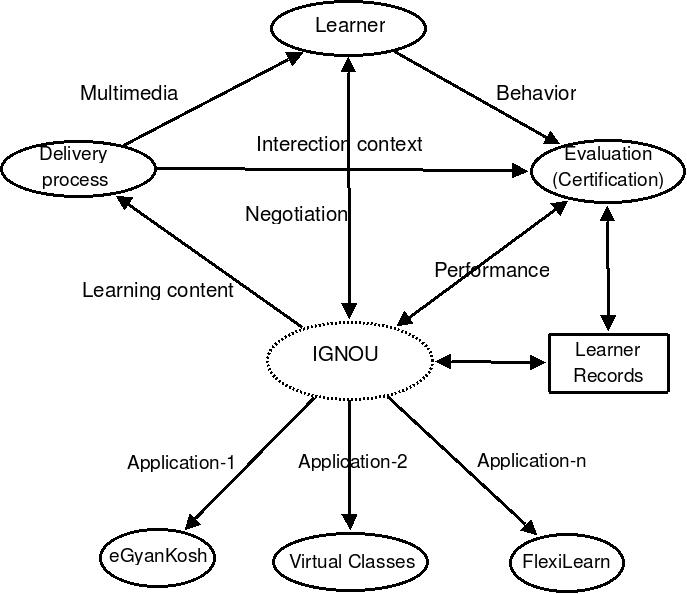
\includegraphics[scale=.5]{flexi1.jpeg}
 % flexi1.jpeg: 687x594 pixel, 72dpi, 24.24x20.95 cm, bb=0 0 687 594
 \caption{FlexiLearn Distributed System Architecture}
\end{figure}
\begin{figure}[htb]
 \centering
 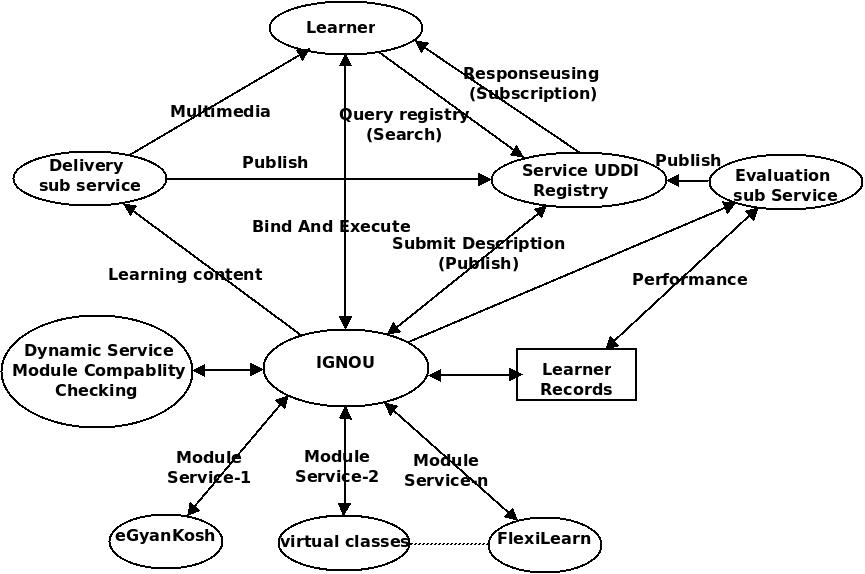
\includegraphics[scale=.5]{ignousoa2.jpeg}
 % flexisoajournal.jpeg: 898x583 pixel, 72dpi, 31.68x20.57 cm, bb=0 0 898 583
 \caption{FexiLearn system in IEEE LTSA mapped in SOA}
\end{figure}

\section{Limitation of present Flexilearn system}
\blindtext
\section{Comparision of IGNOU online services in terms of composition of services}
\blindtext
\section{Security Capacity in the Proposed Model in SOA}
\blindtext
\subsection{Approach To Protecting Services}
\blindtext

\subsubsection{Protect services from the outside at deployment time by using WSM (web service manager) solutions}
\blindtext
\subsubsection{Protect services from the inside by building security into software development process}
Devloper of e-Learning services must validate the input usually in XML document format. Various types of attacks are, buffer overflow, SQL injection, XML injection,
and XPath exploits. Static analytical tools are used for identifying such vulnerabilities.
\subsubsection{Simulation of known attack patterns and fixing vulnerabilities}
Dynamic analysis tools are used during the query and analysis (QA) process to
test, verify and validate the actual deployment. Stress-testing of SOA applications
calls for designing different attack patterns. Vulnerabilities may be uncovered and
resolved before deployment. This may be considered under preventive security
maintenance.
\subsubsection{Monitoring WSM solutions}
\blindtext
\subsection{Protecting Services from the Outside}
\blindtext

